% !TeX root = ../dissertation.tex

\cleardoublepage

\nocite{*}
\printbibliography[heading=bibintoc]

\appendix

\cleardoublepage

\chapter{Extended optimised compiler example} \label{appendix-example}

We will consider the clamp function which calculates

\[
    \text{clamp}(h, l, x) = \begin{cases*}
        h & \text{if }h < x  \\
        l & \text{if }l > x  \\
        x & \text{otherwise} \\
    \end{cases*}
\]

In OCaml it can be defined

\begin{minted}{ocaml}
(% clamp : int -> int -> int %)
let clamp h l (x : int) =
  if h < x then
    h
  else if l > x then
    l
  else
    x
\end{minted}

\section{Basic blocks}

It is compiled to bytecode which basic block conversions parses to:

% \begin{verbatim}
% Arity: 3
% Max stack size: 4
% 
% # Block 0 (stack_start = 3)
% Acc(2)
% Push
% Acc(1)
% IntCmp(Lt)
% Exit: BranchIf { then_block: 1, else_block: 2 }
% 
% # Block 1 (stack_start = 3)
% Acc(0)
% Exit: Return(3)
% 
% # Block 2 (stack_start = 3)
% Acc(2)
% Push
% Acc(2)
% IntCmp(Gt)
% Exit: BranchIf { then_block: 3, else_block: 4 }
% 
% # Block 3 (stack_start = 3)
% Acc(1)
% Exit: Return(3)
% 
% # Block 4 (stack_start = 3)
% Acc(2)
% Exit: Return(3)
% \end{verbatim}


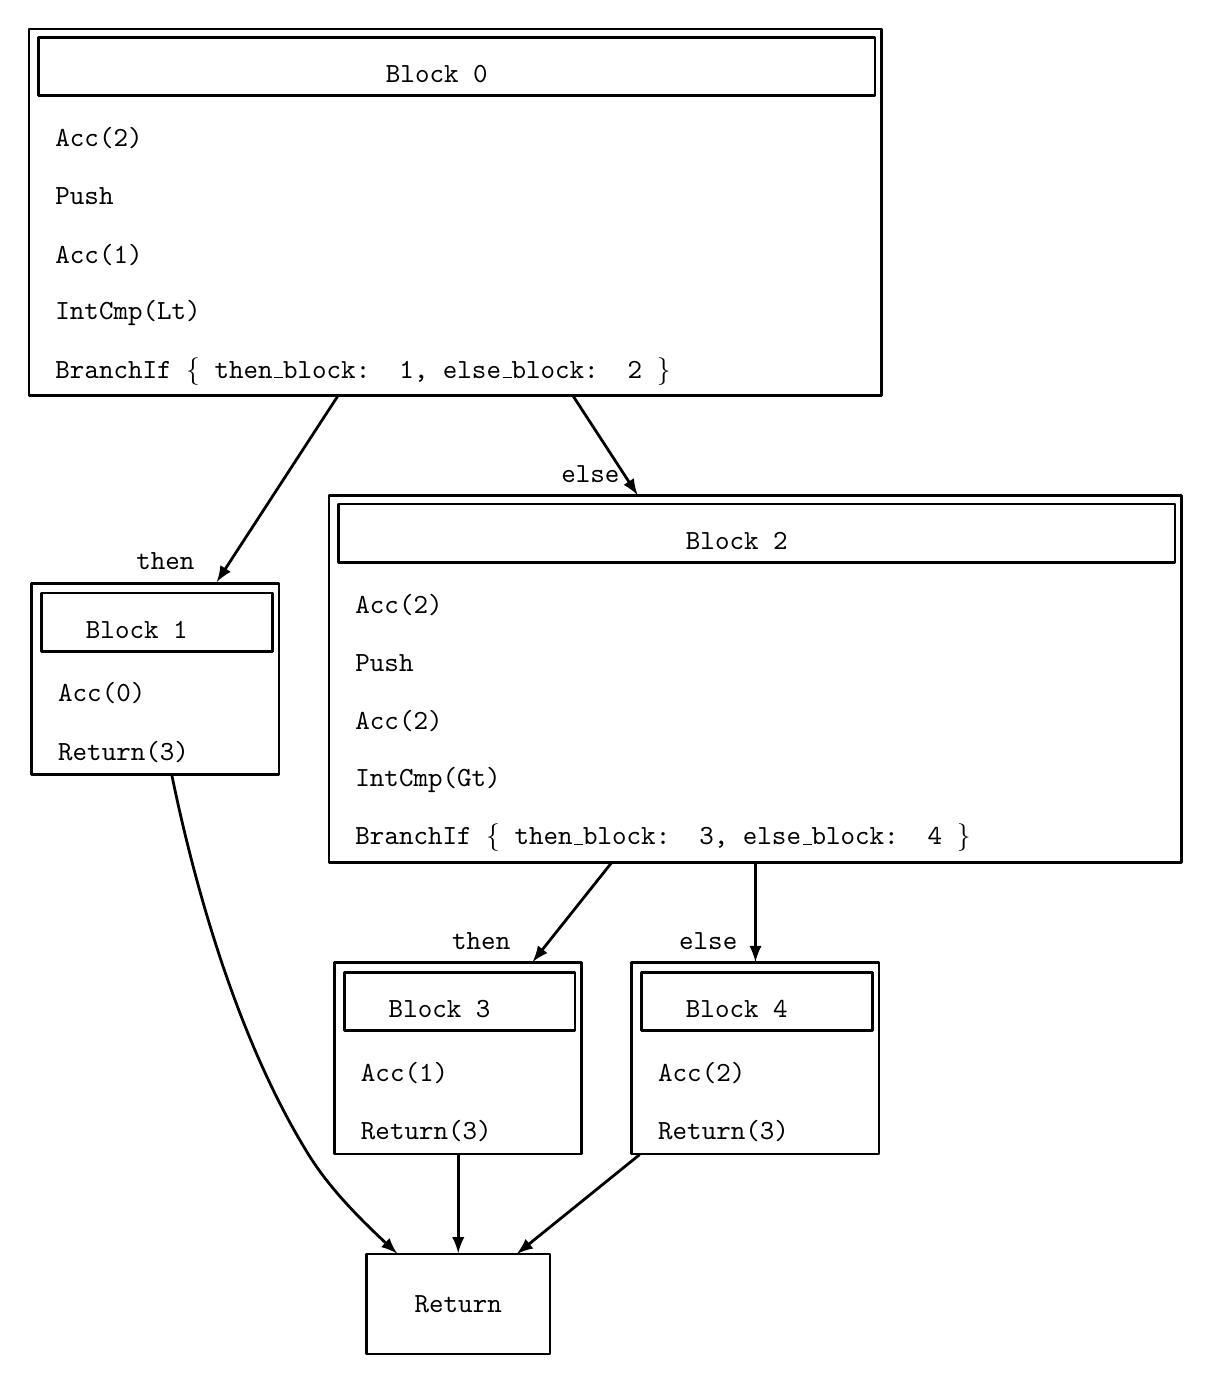
\begin{tikzpicture}[>=latex,line join=bevel,]
  \pgfsetlinewidth{1bp}
\ttfamily%
\pgfsetcolor{black}
  % Edge: n0 -> n1
  \draw [->] (111.13bp,344.87bp) .. controls (98.328bp,325.2bp) and (84.615bp,304.12bp)  .. (67.561bp,277.91bp);
  \definecolor{strokecol}{rgb}{0.0,0.0,0.0};
  \pgfsetstrokecolor{strokecol}
  \draw (49.061bp,285.41bp) node { then};
  % Edge: n0 -> n2
  \draw [->] (195.87bp,344.87bp) .. controls (201.65bp,335.99bp) and (207.61bp,326.82bp)  .. (219.07bp,309.22bp);
  \draw (202.07bp,316.72bp) node { else};
  % Edge: n1 -> return
  \draw [->] (51.405bp,208.35bp) .. controls (58.789bp,172.52bp) and (73.825bp,115.14bp)  .. (100.5bp,72.0bp) .. controls (107.02bp,61.458bp) and (116.07bp,51.486bp)  .. (132.53bp,36.158bp);
  % Edge: n2 -> n3
  \draw [->] (209.57bp,176.72bp) .. controls (202.07bp,167.29bp) and (194.52bp,157.81bp)  .. (181.28bp,141.16bp);
  \draw (162.78bp,148.66bp) node { then};
  % Edge: n2 -> n4
  \draw [->] (261.5bp,176.72bp) .. controls (261.5bp,168.06bp) and (261.5bp,159.36bp)  .. (261.5bp,141.16bp);
  \draw (244.5bp,148.66bp) node { else};
  % Edge: n3 -> return
  \draw [->] (154.5bp,71.809bp) .. controls (154.5bp,63.365bp) and (154.5bp,54.41bp)  .. (154.5bp,36.297bp);
  % Edge: n4 -> return
  \draw [->] (219.82bp,71.809bp) .. controls (207.64bp,61.961bp) and (194.6bp,51.416bp)  .. (175.6bp,36.059bp);
  % Node: n0
\begin{scope}
  \definecolor{strokecol}{rgb}{0.0,0.0,0.0};
  \pgfsetstrokecolor{strokecol}
  \draw (3.5bp,453.0bp) -- (3.5bp,474.0bp) -- (304.5bp,474.0bp) -- (304.5bp,453.0bp) -- cycle;
  \draw (124.5bp,460.8bp) node[right] {Block 0};
  \draw (5.5bp,437.8bp) node[right] {Acc(2)  };
  \draw (5.5bp,416.8bp) node[right] {Push  };
  \draw (5.5bp,395.8bp) node[right] {Acc(1)  };
  \draw (5.5bp,374.8bp) node[right] {IntCmp(Lt)  };
  \draw (5.5bp,353.8bp) node[right] {BranchIf \{ then\_block: 1, else\_block: 2 \}  };
  \draw (0.0bp,345.0bp) -- (0.0bp,477.0bp) -- (307.0bp,477.0bp) -- (307.0bp,345.0bp) -- cycle;
\end{scope}
  % Node: n1
\begin{scope}
  \definecolor{strokecol}{rgb}{0.0,0.0,0.0};
  \pgfsetstrokecolor{strokecol}
  \draw (4.5bp,253.0bp) -- (4.5bp,274.0bp) -- (87.5bp,274.0bp) -- (87.5bp,253.0bp) -- cycle;
  \draw (16.5bp,260.8bp) node[right] {Block 1};
  \draw (6.5bp,237.8bp) node[right] {Acc(0)  };
  \draw (6.5bp,216.8bp) node[right] {Return(3)  };
  \draw (1.0bp,208.5bp) -- (1.0bp,277.5bp) -- (90.0bp,277.5bp) -- (90.0bp,208.5bp) -- cycle;
\end{scope}
  % Node: n2
\begin{scope}
  \definecolor{strokecol}{rgb}{0.0,0.0,0.0};
  \pgfsetstrokecolor{strokecol}
  \draw (111.5bp,285.0bp) -- (111.5bp,306.0bp) -- (412.5bp,306.0bp) -- (412.5bp,285.0bp) -- cycle;
  \draw (232.5bp,292.8bp) node[right] {Block 2};
  \draw (113.5bp,269.8bp) node[right] {Acc(2)  };
  \draw (113.5bp,248.8bp) node[right] {Push  };
  \draw (113.5bp,227.8bp) node[right] {Acc(2)  };
  \draw (113.5bp,206.8bp) node[right] {IntCmp(Gt)  };
  \draw (113.5bp,185.8bp) node[right] {BranchIf \{ then\_block: 3, else\_block: 4 \}  };
  \draw (108.0bp,177.0bp) -- (108.0bp,309.0bp) -- (415.0bp,309.0bp) -- (415.0bp,177.0bp) -- cycle;
\end{scope}
  % Node: return
\begin{scope}
  \definecolor{strokecol}{rgb}{0.0,0.0,0.0};
  \pgfsetstrokecolor{strokecol}
  \draw (187.5bp,36.0bp) -- (121.5bp,36.0bp) -- (121.5bp,0.0bp) -- (187.5bp,0.0bp) -- cycle;
  \draw (154.5bp,18.0bp) node {Return};
\end{scope}
  % Node: n3
\begin{scope}
  \definecolor{strokecol}{rgb}{0.0,0.0,0.0};
  \pgfsetstrokecolor{strokecol}
  \draw (113.5bp,116.5bp) -- (113.5bp,137.5bp) -- (196.5bp,137.5bp) -- (196.5bp,116.5bp) -- cycle;
  \draw (125.5bp,124.3bp) node[right] {Block 3};
  \draw (115.5bp,101.3bp) node[right] {Acc(1)  };
  \draw (115.5bp,80.3bp) node[right] {Return(3)  };
  \draw (110.0bp,72.0bp) -- (110.0bp,141.0bp) -- (199.0bp,141.0bp) -- (199.0bp,72.0bp) -- cycle;
\end{scope}
  % Node: n4
\begin{scope}
  \definecolor{strokecol}{rgb}{0.0,0.0,0.0};
  \pgfsetstrokecolor{strokecol}
  \draw (220.5bp,116.5bp) -- (220.5bp,137.5bp) -- (303.5bp,137.5bp) -- (303.5bp,116.5bp) -- cycle;
  \draw (232.5bp,124.3bp) node[right] {Block 4};
  \draw (222.5bp,101.3bp) node[right] {Acc(2)  };
  \draw (222.5bp,80.3bp) node[right] {Return(3)  };
  \draw (217.0bp,72.0bp) -- (217.0bp,141.0bp) -- (306.0bp,141.0bp) -- (306.0bp,72.0bp) -- cycle;
\end{scope}
%
\end{tikzpicture}



\section{Cranelift IR}

My cranelift IR generation produces this:

\begin{verbatim}
function u0:0(r64, r64, r64, r64) -> r64, i64 system_v {
    gv0 = symbol u1:0

block0(v0: r64, v1: r64, v2: r64, v3: r64):
    v4 = null.r64 
    v5 = iconst.i64 0
    v26 -> v5
    v6 = symbol_value.i64 gv0
    v7 = raw_bitcast.i64 v1
    v8 = raw_bitcast.i64 v3
    v9 = ifcmp v7, v8
    v10 = iconst.i64 3
    v11 = iconst.i64 1
    v12 = selectif.i64 slt v9, v10, v11
    v13 = raw_bitcast.r64 v12
    v14 = raw_bitcast.i64 v13
    v15 = icmp_imm eq v14, 1
    brz v15, block1
    jump block2

block1:
    jump block5(v1)

block2:
    v16 = raw_bitcast.i64 v2
    v17 = raw_bitcast.i64 v3
    v18 = ifcmp v16, v17
    v19 = iconst.i64 3
    v20 = iconst.i64 1
    v21 = selectif.i64 sgt v18, v19, v20
    v22 = raw_bitcast.r64 v21
    v23 = raw_bitcast.i64 v22
    v24 = icmp_imm eq v23, 1
    brz v24, block3
    jump block4

block3:
    jump block5(v2)

block4:
    jump block5(v3)

block5(v25: r64):
    return v25, v5
}
\end{verbatim}

\section{Machine code}

The IR is compiled to

\begin{verbatim}
0000000000000000 <clamp>:
   0:	55                   	push   rbp
   1:	48 89 e5             	mov    rbp,rsp
   4:	48 89 f0             	mov    rax,rsi
   7:	49 89 c9             	mov    r9,rcx
   a:	41 b8 03 00 00 00    	mov    r8d,0x3
  10:	bf 01 00 00 00       	mov    edi,0x1
  15:	4c 39 c8             	cmp    rax,r9
  18:	48 89 f8             	mov    rax,rdi
  1b:	49 0f 4c c0          	cmovl  rax,r8
  1f:	bf 01 00 00 00       	mov    edi,0x1
  24:	48 39 f8             	cmp    rax,rdi
  27:	0f 85 2a 00 00 00    	jne    57 <clamp+0x57>
  2d:	48 89 d0             	mov    rax,rdx
  30:	be 03 00 00 00       	mov    esi,0x3
  35:	bf 01 00 00 00       	mov    edi,0x1
  3a:	4c 39 c8             	cmp    rax,r9
  3d:	48 0f 4f fe          	cmovg  rdi,rsi
  41:	be 01 00 00 00       	mov    esi,0x1
  46:	48 39 f7             	cmp    rdi,rsi
  49:	0f 84 0b 00 00 00    	je     5a <clamp+0x5a>
  4f:	48 89 d1             	mov    rcx,rdx
  52:	e9 03 00 00 00       	jmp    5a <clamp+0x5a>
  57:	48 89 f1             	mov    rcx,rsi
  5a:	48 31 d2             	xor    rdx,rdx
  5d:	48 89 c8             	mov    rax,rcx
  60:	48 89 ec             	mov    rsp,rbp
  63:	5d                   	pop    rbp
  64:	c3                   	ret    

\end{verbatim}

Cranelift's simple optimisation passes have performed jump coalescing, live variable analysis and
register allocation
to produce fairly well optimised assembly. My code enabled this by translating uses of the OCaml
stack to its primitive values.

\chapter{Complete benchmark results}

Big table (maybe landscape orientation/multiple pages) with all of the benchmark data.

\chapter{Rust dependencies and their licences} \label{appendix-licence}

Names are according to the SPDX License List. Most dependencies are transitive dependencies
of projects I directly depend on.

\begin{description}
    \item[Apache-2.0 OR Apache-2.0 WITH LLVM-exception OR MIT (2)] \hfill \\ wasi, wasi
    \item[Apache-2.0 OR BSL-1.0 (1)] \hfill \\ ryu
    \item[Apache-2.0 OR MIT (75)] anyhow, arrayvec, autocfg, base64, bitflags, bstr, cc,
          cfg-if, cfg-if, crc32fast, crossbeam-utils, dirs, dissimilar, either, encode\_unicode,
          env\_logger,
          errno, expect-test, gcc, getrandom, getrandom, gimli, hashbrown, heck, hermit-abi,
          humantime,
          indexmap, itertools, itoa, lazy\_static, libc, log, memmap2, object, once\_cell,
          ppv-lite86,
          proc-macro-error, proc-macro-error-attr, proc-macro2, proc-macro2, quote, quote, rand,
          rand\_chacha, rand\_core, rand\_hc, regex, regex-syntax, remove\_dir\_all, rust-argon2,
          rustc-hash,
          serde, serde\_derive, serde\_json, shell-words, smallvec, structopt, structopt-derive,
          syn, syn,
          tempfile, term, terminal\_size, thiserror, thiserror-impl, thread\_local,
          unicode-segmentation,
          unicode-width, unicode-xid, unicode-xid, vec\_map, version\_check, winapi,
          winapi-i686-pc-windows-gnu, winapi-x86\_64-pc-windows-gnu
    \item[Apache-2.0 WITH LLVM-exception (13)] \hfill \\ cranelift, cranelift-bforest,
          cranelift-codegen,
          cranelift-codegen-meta, cranelift-codegen-shared, cranelift-entity, cranelift-frontend,
          cranelift-jit, cranelift-module, cranelift-native, cranelift-object, regalloc,
          target-lexicon
    \item[BSD-2-Clause (2)] \hfill \\ arrayref, mach
    \item[BSD-3-Clause (1)] \hfill \\ prettytable-rs
    \item[CC0-1.0] \hfill \\ constant\_time\_eq
          % \item[LGPL-2.1-only WITH OCaml-LGPL-linking-exception (1)] \hfill \\  ocaml-jit-staticlib
    \item[MIT (20)] \hfill \\ ansi\_term, atty, blake2b\_simd, clap, console, default-env,
          errno-dragonfly, indicatif, nix, number\_prefix, os\_pipe, pretty-hex, redox\_syscall,
          redox\_syscall, redox\_users, region, strsim, strum, strum\_macros, textwrap
    \item[MIT OR Unlicence (8)] \hfill \\ aho-corasick, byteorder, csv, csv-core, memchr,
          regex-automata, termcolor, winapi-util
    \item[MPL-2.0 (3)] \hfill \\ colored, dynasm, dynasmrt
          % \item[N/A (2)] \hfill \\ ocaml-jit-shared, ocaml-jit-tools
\end{description}